\subsection{Aufgabe}

\begin{align*}
    & & x_0 &= 1 \\
    f(x) &= \ln x & f(1) &= 0 \\
    f^{I}(x) &= \frac{1}{x} & f^{I}(1) &= 1 \\
    f^{II}(x) &= -\frac{1}{x^2} & f^{II}(1) &= -1 \\
    f^{III}(x) &= \frac{1 \cdot 2}{x^2} & f^{III}(1) &= 2! \\
    f^{IV}(x) &= -\frac{1 \cdot 2 \cdot 3}{x^4} & f^{IV}(1) &= -1 \cdot 2 \cdot 3 \\
    f^{V}(x) &= \frac{1 \cdot 2 \cdot 3 \cdot 4}{x^5} & f^{V}(1) &= 1 \cdot 2 \cdot 3 \cdot 4 \\
    \\
    f^n(x) &= (-1)^{n+1} \cdot (n-1)! \cdot \frac{1}{x^n} & f^n(1) &= (-1)^{n+1} \cdot (n-1)!
\end{align*}

\begin{align*}
    \ln(x)
    &= (x - 1) &- \frac{1}{2!} (x - 1)^2 &+ \frac{1 \cdot 2}{3!} (x - 1)^3 &- \frac{1 \cdot 2 \cdot 3}{4!} (x - 1)^4 &+ \ldots &+ (-1)^{n+1} \frac{(n-1)!}{n!} \cdot (x - 1)^n &+ \ldots \\
    &= (x - 1) &- \frac{1}{2} (x - 1)^2 &+ \frac{1}{3} (x - 1)^3 &- \frac{1}{4} (x - 1)^4 &+ \ldots &+ \frac{(-1)^{n+1}}{n} (x - 1)^n &+ \ldots
\end{align*}

\begin{align*}
    r_0 = \limtoinfty{n} \left| \frac{a_n}{a_{n+1}} \right|
        = \limtoinfty{n} \left| \frac{\frac{1}{n}}{\frac{1}{n+1}} \right|
        = \limtoinfty{n} \left| \frac{n+1}{n} \right|
        = \limtoinfty{n} \frac{1 + \frac{1}{n}}{1}
        = 1 \\
    \left| x - 1 \right| < 1
\end{align*}


\begin{figure}[H]
    \centering
    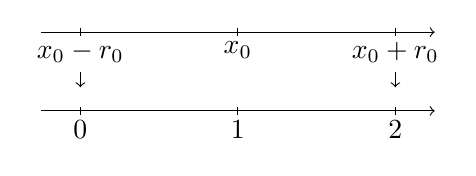
\begin{tikzpicture}
        \draw[->] (-2.5, 0) -- (2.5, 0);
        \node[below] at (-2, 0) {\( x_0 - r_0 \)}; 
        \node[below] at (0, 0) {\( x_0 \)}; 
        \node[below] at (2, 0) {\( x_0 + r_0 \)};

        \draw (-2, 0.05) -- (-2, -0.05); 
        \draw (0, 0.05) -- (0, -0.05); 
        \draw (2, 0.05) -- (2, -0.05); 
        
        \draw[->] (-2, -0.5) -- (-2, -0.7);
        \draw[->] (2, -0.5) -- (2, -0.7);

        \draw[->] (-2.5, -1) -- (2.5, -1);
        \node[below] at (-2, -1) {0}; 
        \node[below] at (0, -1) {1}; 
        \node[below] at (2, -1) {2};

        \draw (-2, -0.95) -- (-2, -1.05); 
        \draw (0, -0.95) -- (0, -1.05); 
        \draw (2, -0.95) -- (2, -1.05); 
    \end{tikzpicture}
\end{figure}

\begin{align*}
    \underline{x_1 = 0:} \\
    P(x_1) &= -1 - \frac{1}{2} (-1)^2 + \frac{1}{3} (-1)^3 - \frac{1}{4} (-1)^4 + \frac{1}{5} (-1)^5 \pm \ldots \\
    &= -1 - \frac{1}{2} - \frac{1}{3} - \frac{1}{4} - \frac{1}{5} - \ldots \\
    &= (-1) \underbrace{\left( 1 + \frac{1}{2} + \frac{1}{3} + \frac{1}{4} + \frac{1}{5} + \ldots \right)}_{\text{harmonische Reihe \(\Rightarrow\) divergent}}
\end{align*}

\begin{align*}
    \underline{x_2 = 2:} \\
    P(x_2) &= \underbrace{1 - \frac{1}{2} + \frac{1}{3} - \frac{1}{4} + \frac{1}{4} - \frac{1}{5} - \frac{1}{6} + \frac{1}{7} \pm \ldots}_{\text{alternierende harmonische Reihe \(\Rightarrow\) bedingt konvergent}}
\end{align*}

Konvergenzradius:

\[
    0 < x \leq 2
\]

Fehlerabschätzung: Abbruch nach viertem Glied

\begin{align*}
    R_6 &= \frac{1}{5} (x - 1)^5 \\
    R_5(1,1) &= \frac{1}{5} (0,1)^5 = 0,000002 \\
    \ln (1,1) &= 0,1 - \frac{1}{2} (0,1)^2 + \frac{1}{3} (0,1)^3 - \frac{1}{4} (0,1)^4 = 0,095308333 \\
    \ln (1,1) &= 0,0953101798
\end{align*}

\[
    \begin{array}{*{12}{c@{\,}}}
        & 0, & 0 & 9 & 5 & 3 & 1 & 0 & 1 & 7 & 9 & 8 \\
        - & 0, & 0 & 9 & 5 & 3 & 0 & 8 & 3 & 3 & 3 & 0 \\
        \hline
        & 0, & 0 & 0 & 0 & 0 & 0 & 1 & 8 & 4 & 6 & 8
    \end{array}
\]
    
\[
    0,0000018468 < 0,000002  
\]
